\documentclass[border=12pt]{standalone}
\usepackage{tikz}
\usepackage{amsmath,amssymb}
\usetikzlibrary{positioning, calc, fit, backgrounds, arrows.meta}

% === COLORS ===
\definecolor{attnblue}{HTML}{4A90D9}
\definecolor{mlporange}{HTML}{E8913A}
\definecolor{compgreen}{HTML}{2EAD6B}
\definecolor{nernstpurp}{HTML}{8E6CC0}
\definecolor{readoutred}{HTML}{D94A5E}
\definecolor{scaffold}{HTML}{999999}
\definecolor{inputcol}{HTML}{6C5CE7}

\newcommand{\dimtag}{\tiny\color{black!50}}

\begin{document}
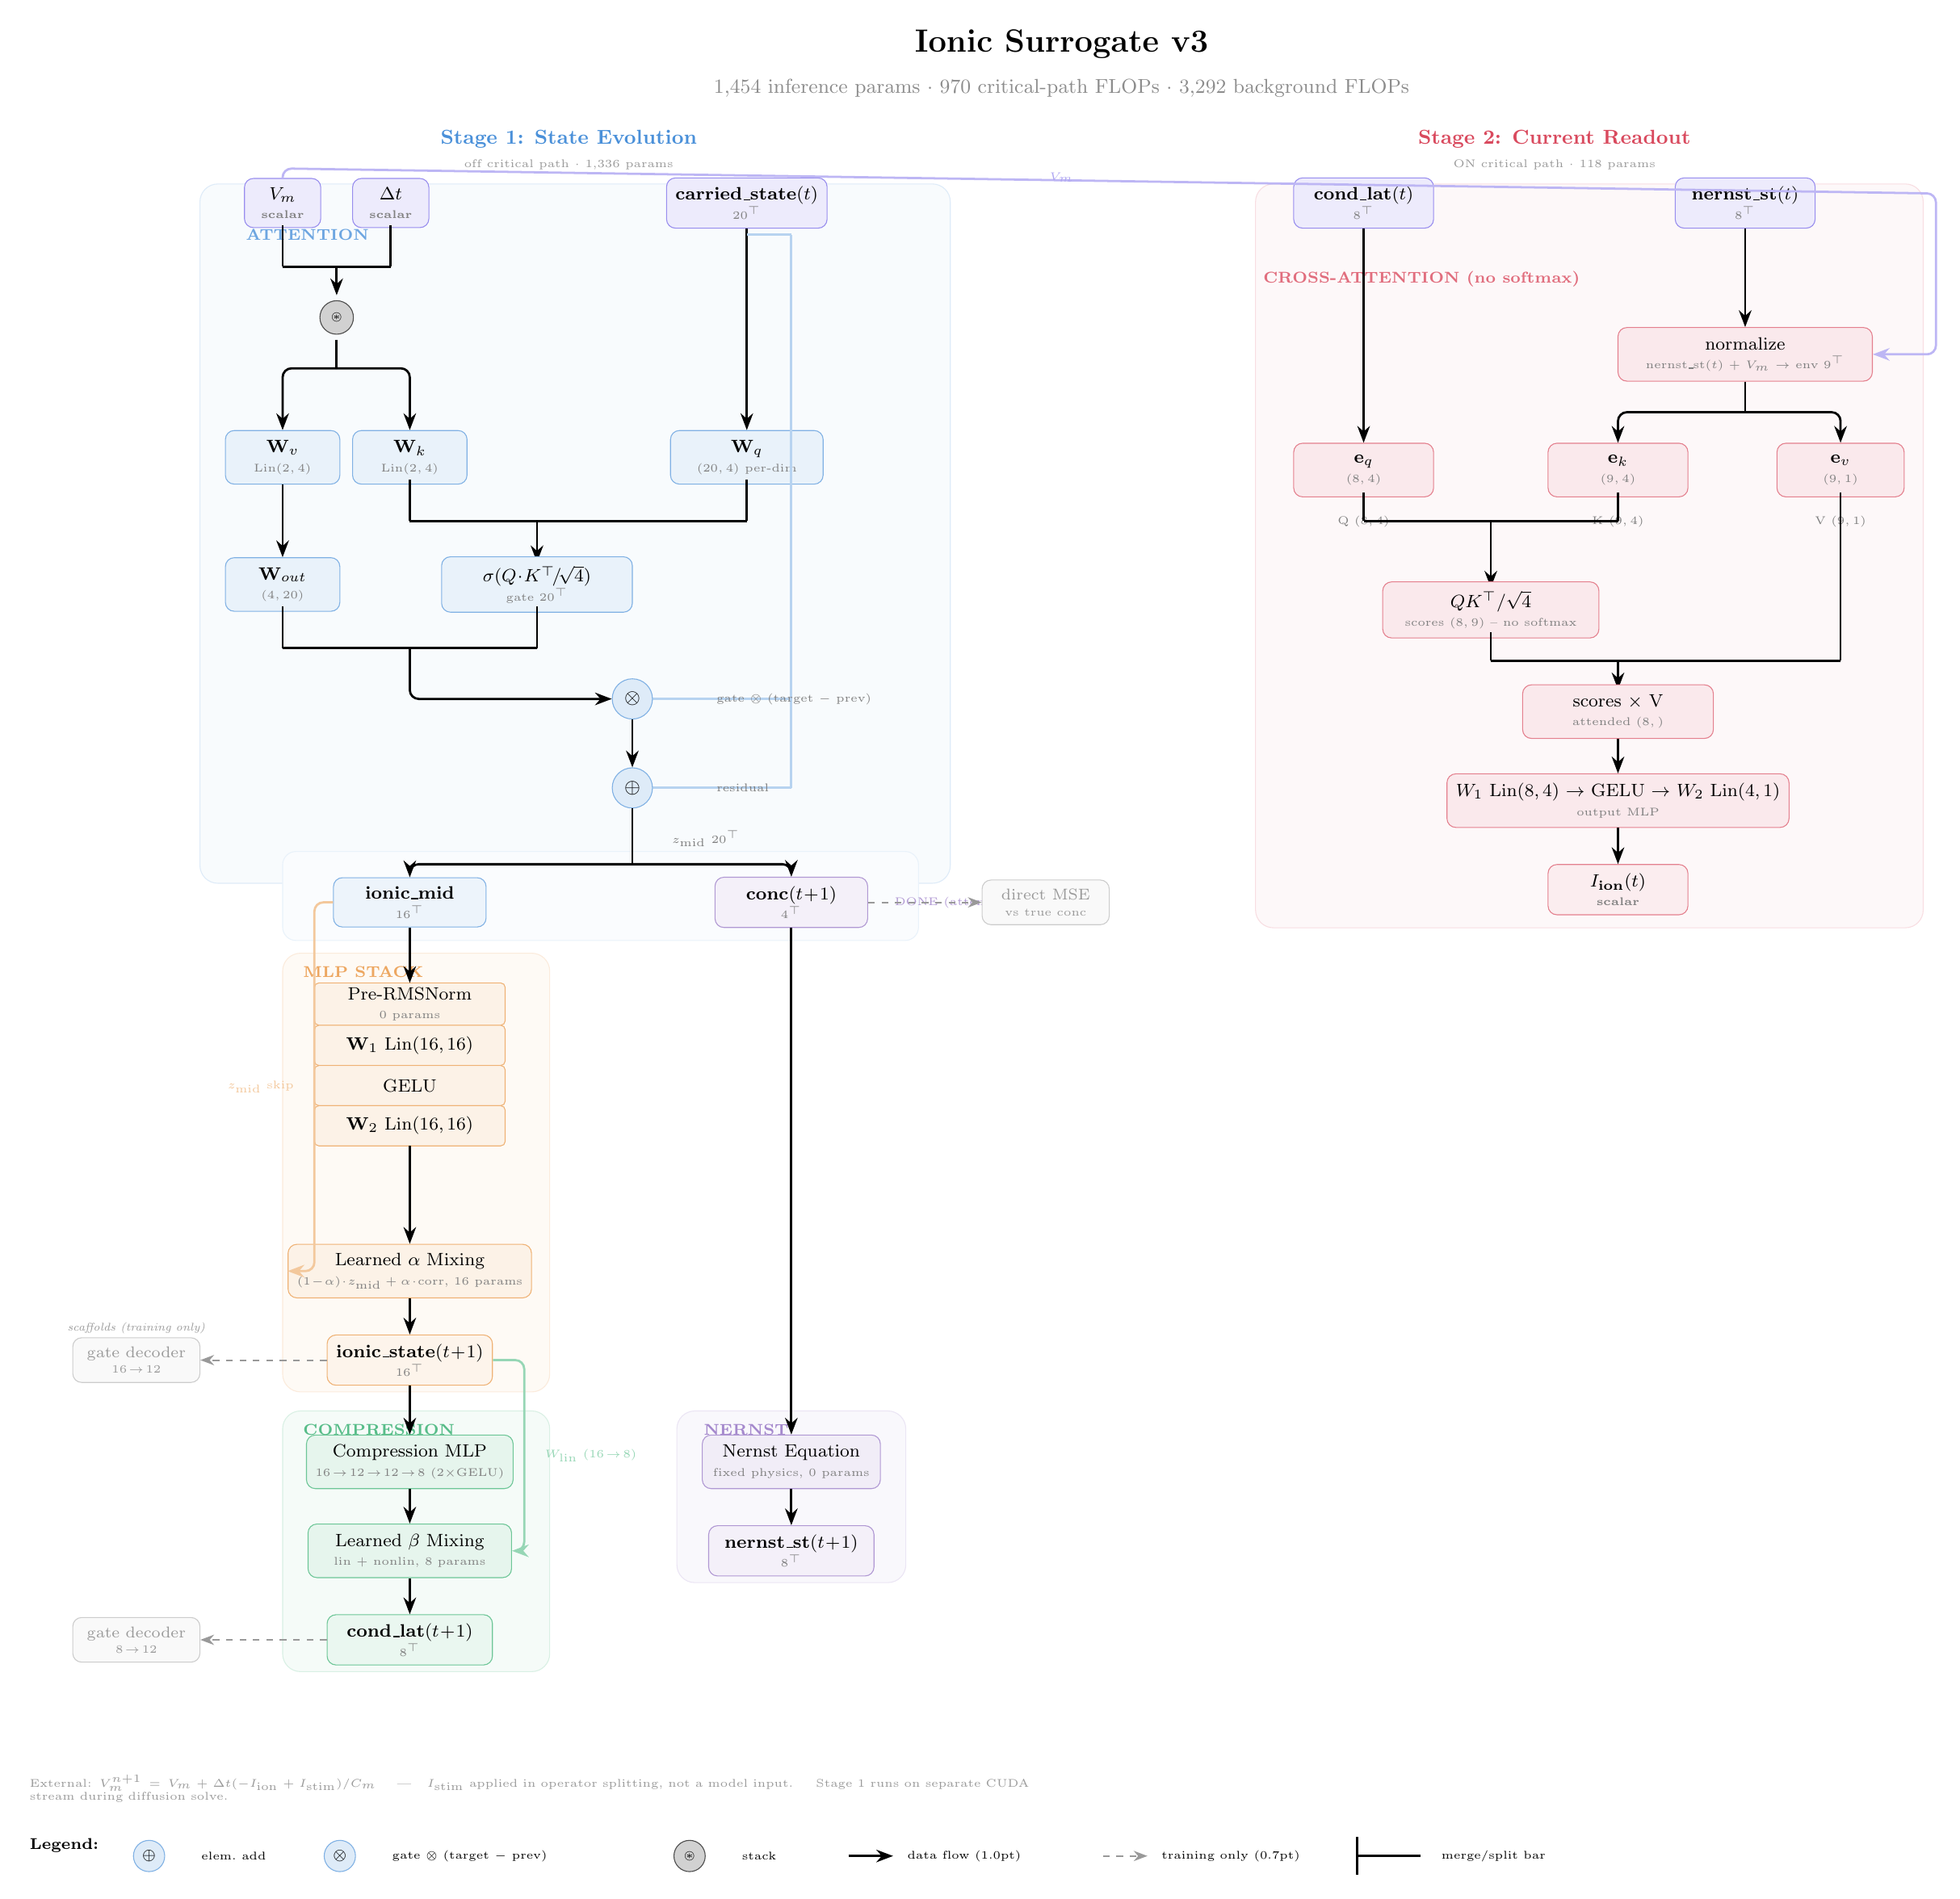
\begin{tikzpicture}[
    >=Stealth,
    every path/.append style={rounded corners=4pt},
    flow/.style={->, line width=1.0pt},
    trunk/.style={line width=1.0pt},
    scaffoldflow/.style={->, line width=0.7pt, dashed, scaffold},
    layer/.style={
        rectangle, draw=#1!70, rounded corners=4pt,
        fill=#1!12, minimum height=2.4em, minimum width=2.2cm,
        align=center, font=\footnotesize, inner sep=4pt
    },
    layer/.default=black,
    mlpblock/.style={
        rectangle, draw=mlporange!70, rounded corners=2pt,
        fill=mlporange!12, minimum height=1.8em, minimum width=3.0cm,
        align=center, font=\footnotesize, inner sep=2pt,
        outer sep=0pt
    },
    inputnode/.style={
        rectangle, draw=inputcol!70, rounded corners=4pt,
        fill=inputcol!12, minimum height=2.2em, minimum width=2.0cm,
        align=center, font=\footnotesize\bfseries, inner sep=4pt
    },
    outputnode/.style={
        rectangle, draw=#1!70, rounded corners=4pt,
        fill=#1!10, minimum height=2.2em, minimum width=2.0cm,
        align=center, font=\footnotesize\bfseries, inner sep=4pt
    },
    outputnode/.default=black,
    op/.style={
        circle, draw=#1!70, fill=#1!18, inner sep=0pt,
        minimum size=1.8em, font=\small\bfseries
    },
    op/.default=black,
    scaffbox/.style={
        rectangle, draw=scaffold!50, rounded corners=4pt,
        fill=scaffold!6, minimum height=2.0em, minimum width=2.0cm,
        align=center, font=\scriptsize\color{scaffold}, inner sep=3pt
    },
    seclabel/.style={font=\scriptsize\bfseries, text=#1!80},
]

% === TITLE ===
\node[font=\Large\bfseries] at (7.75,2.5) {Ionic Surrogate v3};
\node[font=\small, text=black!45] at (7.75,1.8)
    {1,454 inference params $\cdot$ 970 critical-path FLOPs $\cdot$ 3,292 background FLOPs};

% === COLUMN HEADERS ===
\node[font=\small\bfseries, text=attnblue] at (0,1)
    {Stage 1: State Evolution};
\node[font=\tiny, text=black!40] at (0,0.6)
    {off critical path $\cdot$ 1,336 params};

\node[font=\small\bfseries, text=readoutred] at (15.5,1)
    {Stage 2: Current Readout};
\node[font=\tiny, text=black!40] at (15.5,0.6)
    {ON critical path $\cdot$ 118 params};

% === INPUTS ===
\node[inputnode, minimum width=1.2cm] (vm) at (-4.5,0)
    {$V_m$\\[-1pt]{\dimtag scalar}};
\node[inputnode, minimum width=1.2cm] (dt) at (-2.8,0)
    {$\Delta t$\\[-1pt]{\dimtag scalar}};
\node[inputnode, minimum width=2.4cm] (cs) at (2.8,0)
    {carried\_state$(t)$\\[-1pt]{\dimtag $20^\top$}};

\node[inputnode, minimum width=2.2cm] (condR) at (12.5,0)
    {cond\_lat$(t)$\\[-1pt]{\dimtag $8^\top$}};
\node[inputnode, minimum width=2.2cm] (nstR) at (18.5,0)
    {nernst\_st$(t)$\\[-1pt]{\dimtag $8^\top$}};

% === STAGE 1: CROSS-ATTENTION ===
\node[seclabel=attnblue, anchor=west] at (-5.2,-0.5) {ATTENTION};

% --- Vm + dt merge bar -> stack ---
\draw[trunk] (-4.5,-0.35) -- (-4.5,-1);
\draw[trunk] (-2.8,-0.35) -- (-2.8,-1);
\draw[trunk] (-4.5,-1) -- (-2.8,-1);
\node[op=black, minimum size=1.5em] (stack) at (-3.65,-1.8) {\tiny$\circledast$};
\draw[flow] (-3.65,-1) -- (-3.65,-1.45);

% --- ROW A: W_v, W_k, W_q ---
\node[layer=attnblue, minimum width=1.8cm] (wv) at (-4.5,-4)
    {$\mathbf{W}_v$\\[-1pt]{\dimtag Lin$(2,4)$}};
\node[layer=attnblue, minimum width=1.8cm] (wk) at (-2.5,-4)
    {$\mathbf{W}_k$\\[-1pt]{\dimtag Lin$(2,4)$}};
\node[layer=attnblue, minimum width=2.4cm] (wq) at (2.8,-4)
    {$\mathbf{W}_q$\\[-1pt]{\dimtag $(20,4)$ per-dim}};

% stack splits to W_v and W_k
\draw[trunk] (-3.65,-2.15) -- (-3.65,-2.6);
\draw[flow] (-3.65,-2.6) -- (-4.5,-2.6) -- (wv.north);
\draw[flow] (-3.65,-2.6) -- (-2.5,-2.6) -- (wk.north);

% carried_state -> W_q (main trunk)
\coordinate (csbranch) at (2.8,-0.5);
\draw[trunk] (cs.south) -- (csbranch);
\draw[flow] (csbranch) -- (wq.north);

% Skip connection: carried_state -> Hadamard and Add
\draw[trunk, attnblue!40] (csbranch) -- (3.5,-0.5);
\draw[trunk, attnblue!40] (3.5,-0.5) -- (3.5,-7.8);
\draw[flow, attnblue!40] (3.5,-7.8) -- (1,-7.8);
\draw[trunk, attnblue!40] (3.5,-7.8) -- (3.5,-9.2);
\draw[flow, attnblue!40] (3.5,-9.2) -- (1,-9.2);

% --- Q+K merge bar ---
\draw[trunk] (-2.5,-4.35) -- (-2.5,-5);
\draw[trunk] (2.8,-4.35) -- (2.8,-5);
\draw[trunk] (-2.5,-5) -- (2.8,-5);
\draw[flow] (-0.5,-5) -- (-0.5,-5.65);

% --- ROW B: sigma gate + W_out ---
\node[layer=attnblue, minimum width=3.0cm] (siggate) at (-0.5,-6)
    {$\sigma(Q\!\cdot\!K^\top\!/\!\sqrt{4})$\\[-1pt]{\dimtag gate $20^\top$}};
\node[layer=attnblue, minimum width=1.8cm] (wout) at (-4.5,-6)
    {$\mathbf{W}_{out}$\\[-1pt]{\dimtag $(4,20)$}};
\draw[flow] (wv.south) -- (wout.north);

% --- gate + target merge bar ---
\draw[trunk] (-0.5,-6.35) -- (-0.5,-7);
\draw[trunk] (-4.5,-6.35) -- (-4.5,-7);
\draw[trunk] (-4.5,-7) -- (-0.5,-7);

% --- ROW C: Hadamard ---
\node[op=attnblue] (had1) at (1,-7.8) {$\otimes$};
\draw[flow] (-2.5,-7) -- (-2.5,-7.8) -- (had1.west);
\node[font=\tiny, text=black!50, anchor=west] at (2.2,-7.8)
    {gate $\otimes$ (target $-$ prev)};

% --- ROW D: residual add ---
\node[op=attnblue] (add1) at (1,-9.2) {$\oplus$};
\draw[flow] (had1.south) -- (add1.north);
\node[font=\tiny, text=black!50, anchor=west] at (2.2,-9.2)
    {residual};

% --- z_mid label ---
\node[font=\tiny, text=black!50, anchor=west] at (1.5,-10)
    {$z_{\text{mid}}$ $20^\top$};

% === POST-ATTENTION SPLIT ===
\node[outputnode=attnblue, minimum width=2.4cm] (ionicmid) at (-2.5,-11)
    {ionic\_mid\\[-1pt]{\dimtag $16^\top$}};
\node[outputnode=nernstpurp, minimum width=2.4cm] (concout) at (3.5,-11)
    {conc$(t\!+\!1)$\\[-1pt]{\dimtag $4^\top$}};

% Split: add1 straight down, then fork left (ionic) and right (conc)
\draw[trunk] (add1.south) -- (1,-10.4);
\draw[flow] (1,-10.4) -- (-2.5,-10.4) -- (ionicmid.north);
\draw[flow] (1,-10.4) -- (3.5,-10.4) -- (concout.north);

\node[font=\tiny, text=nernstpurp!70, anchor=west] at (5,-11)
    {DONE (attention-only)};

% === MLP STACK ===
\node[seclabel=mlporange, anchor=west] at (-4.3,-12.1)
    {MLP STACK};

\node[mlpblock] (mlp1) at (-2.5,-12.6)
    {Pre-RMSNorm\\[-1pt]{\dimtag 0 params}};
\node[mlpblock, anchor=north] (mlp2) at (mlp1.south)
    {$\mathbf{W}_1$ Lin$(16,16)$};
\node[mlpblock, anchor=north] (mlp3) at (mlp2.south)
    {GELU};
\node[mlpblock, anchor=north] (mlp4) at (mlp3.south)
    {$\mathbf{W}_2$ Lin$(16,16)$};

\draw[flow] (ionicmid.south) -- (mlp1.north);

% === LEARNED ALPHA MIXING ===
\node[layer=mlporange, minimum width=3.6cm] (amix) at (-2.5,-16.8)
    {Learned $\alpha$ Mixing\\[-1pt]{\dimtag $(1\!-\!\alpha)\!\cdot\!z_{\text{mid}} + \alpha\!\cdot\!\text{corr}$, 16 params}};
\draw[flow] (mlp4.south) -- (amix.north);

% z_mid residual skip -> alpha mixing
\draw[flow, mlporange!50] (ionicmid.west) -- (-4,-11) -- (-4,-16.8) -- (amix.west);
\node[font=\tiny, text=mlporange!50, anchor=east] at (-4.2,-13.9)
    {$z_{\text{mid}}$ skip};

% === IONIC STATE OUTPUT ===
\node[outputnode=mlporange, minimum width=2.6cm] (ionicout) at (-2.5,-18.2)
    {ionic\_state$(t\!+\!1)$\\[-1pt]{\dimtag $16^\top$}};
\draw[flow] (amix.south) -- (ionicout.north);

% === COMPRESSION ===
\node[seclabel=compgreen, anchor=west] at (-4.3,-19.3)
    {COMPRESSION};

\node[layer=compgreen, minimum width=3.2cm] (comp) at (-2.5,-19.8)
    {Compression MLP\\[-1pt]{\dimtag $16\!\to\!12\!\to\!12\!\to\!8$ (2$\times$GELU)}};
\draw[flow] (ionicout.south) -- (comp.north);

\node[layer=compgreen, minimum width=3.2cm] (bmix) at (-2.5,-21.2)
    {Learned $\beta$ Mixing\\[-1pt]{\dimtag lin $+$ nonlin, 8 params}};
\draw[flow] (comp.south) -- (bmix.north);

% Linear bypass skip
\draw[flow, compgreen!50] (ionicout.east) -- (-0.7,-18.2) -- (-0.7,-21.2) -- (bmix.east);
\node[font=\tiny, text=compgreen!50, anchor=west] at (-0.5,-19.7)
    {$W_{\text{lin}}$ $(16\!\to\!8)$};

\node[outputnode=compgreen, minimum width=2.6cm] (condout) at (-2.5,-22.6)
    {cond\_lat$(t\!+\!1)$\\[-1pt]{\dimtag $8^\top$}};
\draw[flow] (bmix.south) -- (condout.north);

% === NERNST BRANCH ===
\node[seclabel=nernstpurp, anchor=west] at (2,-19.3)
    {NERNST};

\node[layer=nernstpurp, minimum width=2.8cm] (nernst) at (3.5,-19.8)
    {Nernst Equation\\[-1pt]{\dimtag fixed physics, 0 params}};
\draw[flow] (concout.south) -- (nernst.north);

\node[outputnode=nernstpurp, minimum width=2.6cm] (nstout) at (3.5,-21.2)
    {nernst\_st$(t\!+\!1)$\\[-1pt]{\dimtag $8^\top$}};
\draw[flow] (nernst.south) -- (nstout.north);

% === STAGE 2: CROSS-ATTENTION READOUT ===
\node[seclabel=readoutred, anchor=west] at (10.8,-1.19)
    {CROSS-ATTENTION (no softmax)};

% --- Normalize ---
\node[layer=readoutred, minimum width=4.0cm] (norm2) at (18.5,-2.38)
    {normalize\\[-1pt]{\dimtag nernst\_st$(t)$ $+$ $V_m$ $\to$ env $9^\top$}};
\draw[flow] (nstR.south) -- (norm2.north);

% Vm -> normalize route
\draw[flow, inputcol!45]
    (vm.north) -- ++(0, 0.15) -- (21.5,0.15) -- (21.5,-2.38) -- (norm2.east);
\node[font=\tiny, text=inputcol!55, anchor=south] at (7.75,0.2) {$V_m$};

% --- Embedding row ---
\node[layer=readoutred, minimum width=2.2cm] (eq) at (12.5,-4.2)
    {$\mathbf{e}_q$\\[-1pt]{\dimtag $(8,4)$}};
\node[layer=readoutred, minimum width=2.2cm] (ek) at (16.5,-4.2)
    {$\mathbf{e}_k$\\[-1pt]{\dimtag $(9,4)$}};
\node[layer=readoutred, minimum width=2.0cm] (ev) at (20,-4.2)
    {$\mathbf{e}_v$\\[-1pt]{\dimtag $(9,1)$}};

\draw[flow] (condR.south) -- (eq.north);

% normalize -> e_k and e_v
\coordinate (normsplit) at (18.5,-3.29);
\draw[trunk] (norm2.south) -- (normsplit);
\draw[flow] (normsplit) -- (16.5,-3.29) -- (ek.north);
\draw[flow] (normsplit) -- (20,-3.29) -- (ev.north);

% Dimension labels under embeddings
\node[font=\tiny, text=black!50, anchor=north] at (12.5,-4.8) {Q $(8,4)$};
\node[font=\tiny, text=black!50, anchor=north] at (16.5,-4.8) {K $(9,4)$};
\node[font=\tiny, text=black!50, anchor=north] at (20,-4.8) {V $(9,1)$};

% --- Q + K merge bar -> scores ---
\draw[trunk] (12.5,-4.55) -- (12.5,-5);
\draw[trunk] (16.5,-4.55) -- (16.5,-5);
\draw[trunk] (12.5,-5) -- (16.5,-5);
\draw[flow] (14.5,-5) -- (14.5,-6.05);

\node[layer=readoutred, minimum width=3.4cm] (scores) at (14.5,-6.4)
    {$Q K^\top / \sqrt{4}$\\[-1pt]{\dimtag scores $(8,9)$ -- no softmax}};

% --- scores + V merge bar -> attended ---
\draw[trunk] (14.5,-6.75) -- (14.5,-7.2);
\draw[trunk] (20,-4.55) -- (20,-7.2);
\draw[trunk] (14.5,-7.2) -- (20,-7.2);
\draw[flow] (16.5,-7.2) -- (16.5,-7.65);

\node[layer=readoutred, minimum width=3.0cm] (attn) at (16.5,-8)
    {scores $\times$ V\\[-1pt]{\dimtag attended $(8,)$}};

% --- Output MLP ---
\node[layer=readoutred, minimum width=4.2cm] (omlp) at (16.5,-9.4)
    {$W_1$ Lin$(8,4)$ $\to$ GELU $\to$ $W_2$ Lin$(4,1)$\\[-1pt]{\dimtag output MLP}};
\draw[flow] (attn.south) -- (omlp.north);

% --- I_ion output ---
\node[outputnode=readoutred, minimum width=2.2cm] (iion) at (16.5,-10.8)
    {$I_{\text{ion}}(t)$\\[-1pt]{\dimtag scalar}};
\draw[flow] (omlp.south) -- (iion.north);

% === SCAFFOLD DECODERS ===
\node[font=\tiny\itshape, text=scaffold] at (-6.8,-17.7)
    {scaffolds (training only)};

\node[scaffbox] (sdec1) at (-6.8,-18.2)
    {gate decoder\\[-1pt]{\tiny $16\!\to\!12$}};
\draw[scaffoldflow] (ionicout.west) -- (sdec1.east);

\node[scaffbox] (sdec2) at (-6.8,-22.6)
    {gate decoder\\[-1pt]{\tiny $8\!\to\!12$}};
\draw[scaffoldflow] (condout.west) -- (sdec2.east);

\node[scaffbox] (smse) at (7.5,-11)
    {direct MSE\\[-1pt]{\tiny vs true conc}};
\draw[scaffoldflow] (concout.east) -- (smse.west);

% === STAGE BACKGROUNDS ===
\begin{scope}[on background layer]
    \node[fit={(-5.8, 0.3)(6, -10.7)},
          fill=attnblue!4, draw=attnblue!18,
          rounded corners=8pt, inner sep=0pt] {};
    \node[fit={(-4.5, -10.2)(5.5, -11.6)},
          fill=attnblue!3, draw=attnblue!12,
          rounded corners=6pt, inner sep=0pt] {};
    \node[fit={(-4.5, -11.8)(-0.3, -18.7)},
          fill=mlporange!5, draw=mlporange!18,
          rounded corners=8pt, inner sep=0pt] {};
    \node[fit={(-4.5, -19)(-0.3, -23.1)},
          fill=compgreen!5, draw=compgreen!18,
          rounded corners=8pt, inner sep=0pt] {};
    \node[fit={(1.7, -19)(5.3, -21.7)},
          fill=nernstpurp!5, draw=nernstpurp!18,
          rounded corners=8pt, inner sep=0pt] {};
    \node[fit={(10.8, 0.3)(21.3, -11.4)},
          fill=readoutred!4, draw=readoutred!18,
          rounded corners=8pt, inner sep=0pt] {};
\end{scope}

% === ANNOTATIONS ===
\node[font=\tiny, text=black!40, anchor=north west, text width=16cm]
    at (-8.6,-24.6)
    {External: $V_m^{n+1} = V_m + \Delta t(-I_{\text{ion}} + I_{\text{stim}})/C_m$
    \quad---\quad $I_{\text{stim}}$ applied in operator splitting, not a model input.
    \quad Stage 1 runs on separate CUDA stream during diffusion solve.};

% === LEGEND ===
\node[font=\scriptsize\bfseries, anchor=north west] at (-8.6,-25.6) {Legend:};
\node[op=attnblue, minimum size=1.4em, font=\scriptsize\bfseries]
    at (-6.6,-26) {$\oplus$};
\node[font=\tiny, anchor=west] at (-5.9,-26) {elem.\ add};
\node[op=attnblue, minimum size=1.4em, font=\scriptsize\bfseries]
    at (-3.6,-26) {$\otimes$};
\node[font=\tiny, anchor=west] at (-2.9,-26)     {gate $\otimes$ (target $-$ prev)};
\node[op=black, minimum size=1.4em, font=\tiny\bfseries]
    at (1.9,-26) {$\circledast$};
\node[font=\tiny, anchor=west] at (2.6,-26) {stack};
\draw[flow] (4.4,-26) -- ++(0.7, 0);
\node[font=\tiny, anchor=west] at (5.2,-26) {data flow (1.0pt)};
\draw[scaffoldflow] (8.4,-26) -- ++(0.7, 0);
\node[font=\tiny, anchor=west] at (9.2,-26) {training only (0.7pt)};
\draw[trunk] (12.4,-25.7) -- (12.4,-26.3);
\draw[trunk] (12.4,-26) -- (13.4,-26);
\node[font=\tiny, anchor=west] at (13.6,-26) {merge/split bar};

\end{tikzpicture}
\end{document}